
\documentclass[runningheads]{llncs}

% to have bookmarks in pdf
% remove for final version
\usepackage[open,openlevel=5]{bookmark}
\setcounter{tocdepth}{5}

\usepackage{graphicx}
% Used for displaying a sample figure. If possible, figure files should
% be included in EPS format.
%

\graphicspath{{./images/}}

\usepackage{hyperref}
% If you use the hyperref package, please uncomment the following line
% to display URLs in blue roman font according to Springer's eBook style:
\renewcommand\UrlFont{\color{blue}\rmfamily}

%\usepackage{courier}
\usepackage{listings, color}
\hypersetup{
  colorlinks   = true,
  linkcolor  = blue,
  citecolor  = blue,
  urlcolor   = blue
}

% latin modern, no more bitmap fonts in pdf
\usepackage{lmodern}
%\usepackage{newtxtext}
%\usepackage{newtxmath}
\usepackage[zerostyle=b,scaled=.88]{newtxtt}

% nicer bold
\renewcommand{\bfdefault}{b}%


% make paragraph headings bold instead of italics
\renewcommand{\paragraph}{\textbf}%

\definecolor{dkgreen}{rgb}{0,0.6,0}
\definecolor{gray}{rgb}{0.5,0.5,0.5}
\definecolor{mauve}{rgb}{0.58,0,0.82}

\lstdefinestyle{scala}{
  language=scala,
  basicstyle=\footnotesize\ttfamily,
%  basicstyle=\scriptsize\ttfamily, % kai: temporary 
  breaklines=true,
  keywordstyle=\color{blue},
  commentstyle=\color{dkgreen},
  numbers=left,
  %frame=single, % Border around box
  %numbersep=-7pt,
  numberstyle=\color{gray},
  stringstyle=\color{mauve}
}

\lstdefinestyle{stainless}{
  numbers=none,
  breaklines=true,
  breakautoindent=true,
  breakindent=63pt,
  basicstyle=\footnotesize\ttfamily
}
 
\newcommand{\todo}[1]{{\par \color{red}#1}}


\begin{document}

\title{Towards Verifying the Bitcoin-S Library}

\author{Ramon Boss \and Kai Brünnler \and Anna Doukmak}

\authorrunning{R. Boss et al.}
\institute{Bern University of Applied Sciences, CH-2501 Biel, Switzerland
\email{ramon.boss@outlook.com, kai.bruennler@bfh.ch,\\anna.doukmak@gmail.com}}

\maketitle             

\begin{abstract}
  We try to verify properties of the bitcoin-s library, a Scala
  implementation of parts of the Bitcoin protocol. We use the
  Stainless verifier which supports programs in a subset of Scala
  called \emph{Pure Scala}. We first try to verify the property that
  regular transactions do not create new money. It turns out that
  there is too much code involved that lies outside of the supported
  fragment to make this feasible. However, in the process we find and
  fix a bug in bitcoin-s. We then turn to a much simpler property:
  that adding zero satoshis to a given amount of satoshis yields the
  given amount of satoshis. Here as well a significant part of the
  relevant code lies outside of the supported fragment. We perform a
  series of equivalent transformations on it until we arrive at code that we
  successfully verify. In that process we find and fix a second bug in
  bitcoin-s.

\keywords{Bitcoin  \and Scala \and Bitcoin-S \and Stainless.}
\end{abstract}



\section{Introduction}

For software handling cryptocurrency, correctness is clearly crucial.
However, even in very well-tested software such as Bitcoin Core,
serious bugs occur. The most recent example is the bug found in
September 2018 \cite{cve201817144} which essentially allowed to
arbitrarily create new coins. Such software is thus a worthwhile
target for formal verification. In this work, we set out to verify
properties of the bitcoin-s library with the Stainless verifier.

\paragraph{The Bitcoin-S Library.} The bitcoin-s library is an
implementation of parts of the Bitcoin protocol in Scala
\cite{BitcoinS:website,BitcoinS:github}. In particular, it allows to
serialize, deserialize, sign and validate Bitcoin transactions. The library
uses immutable data structures and algebraic data types but is not
written with formal verification in mind. According to the website,
the library is used in production, handling significant amounts of
cryptocurrency each day \cite{BitcoinS:website}.

\paragraph{The Stainless Verifier.} Stainless is the successor of the
Leon verifier
\cite{DBLP:conf/ecoop/BlancKKS13,DBLP:conf/pldi/VoirolKK15,DBLP:conf/pldi/BlancK15}
and is developed at EPF Lausanne \cite{Stainless:github}. It is
intended to be used by programmers without training in formal
verification. To facilitate that, it accepts specifications written in
the programming language itself (Scala). Also, it focusses on
counterexample finding in addition to proving
correctness. Counterexamples are useful to programmers while
correctness proofs are not -- correctness is obvious or does not hold,
and often both at the same time.

The example in Figure~\ref{fig:factorial} adapted from the Stainless
documentation \cite{Stainless:documentation} shows how the verifier is
used. Notice how a precondition is specified using \emph{require} and
a postcondition using \emph{ensuring}.

\begin{figure}
\begin{lstlisting}[style=scala]
  def factorial(n: Int): Int = {
      require(n >= 0)
      if (n == 0) {
        1
      } else {
        n * factorial(n - 1)
      }
  } ensuring(res => res >= 0)
\end{lstlisting}
	\caption{Factorial program with specification}
	\label{fig:factorial}
\end{figure}
Our function does not satisfy the specification. An overflow in the
32-bit Int leads to a negative result for the input 17, as Stainless
reports in Figure~\ref{fig:failed}. Changing the type from Int to
BigInt will result in a successful verification.

\begin{figure}
	\centering
		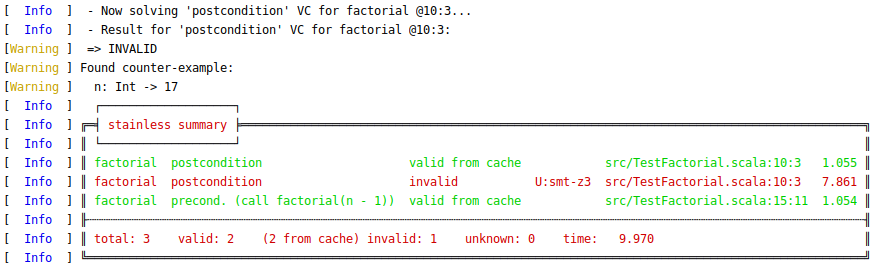
\includegraphics[width=\textwidth]{output1.png}
	\caption{Stainless output for the factorial program}
	\label{fig:failed}
\end{figure}


\paragraph{The Pure Scala Fragment.} The Scala fragment supported by
Stainless is described in the Stainless documentation
\cite{Stainless:documentation} in the section
\href{https://epfl-lara.github.io/stainless/purescala.html}{Pure
  Scala}.

It comprises algebraic data types in the form of abstract classes,
case classes and case objects, objects for grouping classes and
functions, boolean expressions with short-circuit interpretation,
generics with invariant type parameters, default values of function
parameters, pattern matching, local and anonymous classes and more.
  
In addition to Pure Scala Stainless also supports some imperative
features, such as using a (mutable) variable in a local scope of a
function and while loops. They turn out not to be relevant for the
current work.

What will turn out to be more relevant for us are the Scala features
which Stainless does not support, such as: (concrete) class
definitions, inheritance by objects, abstract type members, and inner
classes in case objects.

Also, Stainless has its own library of some core data types and
functions which need to be mapped correctly to functions inside of the
SMT solver that Stainless ultimately relies on. Those data types in
general do not have all the methods of the Scala data types. For
example, the BigInt type in Scala has methods for bitwise operations
while the BigInt type in Stainless does not.

\paragraph{Outline and Properties to Verify.} In the next section we
try to verify the property that a regular (non-coinbase) transaction
can not generate new coins. We call it the \emph{no-inflation
  property}. Trying to verify it, we uncover and fix a bug in the
bitcoin-s library. We then find that there is too much code involved
that lies outside of the supported fragment to currently make this
verification feasible. So we turn to a simpler property to verify. The
simplest possible property we can think of is the fact that adding
zero satoshis to a given amount of satoshis yields the given amount of
satoshis. We call it the \emph{addition-with-zero property} and we try
to verify it in Section~3. Here as well we see that a significant part
of the code lies outside of the supported fragment. We perform a
  series of equivalent transformations on it until we arrive at code that we
  successfully verify. In that process we find and fix a second bug in
  bitcoin-s.


\section{The No-Inflation Property}

\begin{figure}
\begin{lstlisting}[style=scala]
/**
  * Checks the validity of a transaction in accordance to bitcoin core's CheckTransaction function
  * https://github.com/bitcoin/bitcoin/blob/f7a21dae5dbf71d5bc00485215e84e6f2b309d0a/src/main.cpp#L939.
  */
def checkTransaction(transaction: Transaction): Boolean = {
  val inputOutputsNotZero =
    !(transaction.inputs.isEmpty || transaction.outputs.isEmpty)
  val txNotLargerThanBlock = transaction.bytes.size < Consensus.maxBlockSize
  val outputsSpendValidAmountsOfMoney = !transaction.outputs.exists(o =>
    o.value < CurrencyUnits.zero || o.value > Consensus.maxMoney)

  val outputValues = transaction.outputs.map(_.value)
  val totalSpentByOutputs: CurrencyUnit =
    outputValues.fold(CurrencyUnits.zero)(_ + _)
  val allOutputsValidMoneyRange = validMoneyRange(totalSpentByOutputs)
  val prevOutputTxIds = transaction.inputs.map(_.previousOutput.txId)
  val noDuplicateInputs = prevOutputTxIds.distinct.size == prevOutputTxIds.size

  val isValidScriptSigForCoinbaseTx = transaction.isCoinbase match {
    case true =>
      transaction.inputs.head.scriptSignature.asmBytes.size >= 2 &&
        transaction.inputs.head.scriptSignature.asmBytes.size <= 100
    case false =>
      //since this is not a coinbase tx we cannot have any empty previous outs inside of inputs
      !transaction.inputs.exists(_.previousOutput == EmptyTransactionOutPoint)
  }
  inputOutputsNotZero && txNotLargerThanBlock && outputsSpendValidAmountsOfMoney && noDuplicateInputs &&
  allOutputsValidMoneyRange && noDuplicateInputs && isValidScriptSigForCoinbaseTx
}
\end{lstlisting}
  
  \caption{The \texttt{checkTransaction} function}
  \label{fig:checktrans}
\end{figure}


A crucial function for the verification of the no-inflation property
is the function which validates transactions: the
\texttt{checkTransaction} function in the ScriptInterpreter object,
shown in Figure~\ref{fig:checktrans}. It takes a transaction and if
some basic checks succeed returns true, otherwise false. For example,
one of those checks is that both the list of inputs and list of
outputs need to be non-empty.

To better understand the validation of a transaction in bitcoin-s, it
is useful to review how transactions are represented and created.

\paragraph{Creating a Transaction.} The code in this subsection is
adapted from the bitcoin-s documentation. To create a transaction, we
first need some coins -- an unspent transaction output. We could load
an actual unspent transaction output from the bitcoin network, but we
create one manually in order to see this process. So we first create
an (invalid) transaction with one output in Figure~\ref{fig:prevtx}.

\begin{figure}
\begin{lstlisting}[style=scala]
  val privKey = ECPrivateKey.freshPrivateKey
  val creditingSPK = P2PKHScriptPubKey(pubKey = privKey.publicKey)

  val amount = Satoshis(Int64(10000))

  val utxo = TransactionOutput(currencyUnit = amount, scriptPubKey = creditingSPK)

  val prevTx = BaseTransaction(
    version = Int32.one,
    inputs = List.empty,
    outputs = List(utxo),
    lockTime = UInt32.zero
  )
\end{lstlisting}
  
  \caption{Creating a transaction output to spend}
  \label{fig:prevtx}
\end{figure}

We first create a keypair, then a lock script with its public key,
then the amount of satoshis, then a transaction output (utxo) for that
amount and locked with that script. Finally we create the actual
transaction with that output and no inputs. Of course, that is not a
valid transaction, because it creates coins out of nothing. In
particular, checkTransaction(prevTx) returns false, simply because the
list of inputs is empty.

\begin{figure}
\begin{lstlisting}[style=scala]
  val outPoint = TransactionOutPoint(prevTx.txId, UInt32.zero)

  val utxoSpendingInfo = BitcoinUTXOSpendingInfo(
    outPoint = outPoint,
    output = utxo,
    signers = List(privKey),
    redeemScriptOpt = None,
    scriptWitnessOpt = None,
    hashType = HashType.sigHashAll
  )

  val utxos = List(utxoSpendingInfo)

  val destinationAmount = Satoshis(Int64(5000))

  val destinationSPK = P2PKHScriptPubKey(pubKey = ECPrivateKey.freshPrivateKey.publicKey)

  val destinations = List(
    TransactionOutput(currencyUnit = destinationAmount, scriptPubKey = destinationSPK)
  )

  val feeRate = SatoshisPerByte(Satoshis.one)

  val networkParams = RegTest // some static values for testing

  val txBuilderF: Future[BitcoinTxBuilder] = BitcoinTxBuilder(
    destinations = destinations, 
    utxos = utxos,               
    feeRate = feeRate,           
    changeSPK = creditingSPK,    // where to send the change
    network = networkParams      
  )

  val txF: Future[Transaction] = txBuilderF.flatMap(_.sign)

  val tx: Transaction = Await.result(txF, 1 second)
\end{lstlisting}
  \caption{Creating a transaction}
  \label{fig:tx}
\end{figure}

Now that we have a transaction output, we create a transaction to
spend it.

First, we need a so-called \emph{out point}, which points to an output
of a previous transaction. The second parameter is the index of the
referenced output. Here we use zero because the previous transaction
has only one output (with index zero).

Second, we need some information on how to spend the utxo from the
previous transaction, in particular, how to sign the transaction to
allow this. That is the information needed to create a transaction
input, so essentially a transaction input.

Third, we assemble the list of transaction inputs, in our case just one.

Fourth, we set the amount of satoshis that we want to spend. The Int64
class emulates C data types in Scala, and we will look at it more in
the next section.

Fifth, we create a lock script to send the coins to. To be supremely
secure, we use a public key derived from a private key we immediately
forget.

Sixth, we create our list of transaction outputs.

Seventh and eighth, we define the fee rate and some bitcoin network parameters.  

Nineth, we create a transaction builder with those data.

Tenth, we tell the transaction builder to start signing the transaction.

Finally, we get the actual signed transaction. We could serialize it
and send it to the Bitcoin network. We can also pass it to the
checkTransaction function, which will return true.

\paragraph{A Bug in the checkTransaction Function.} Note lines 16 and
17 of the checkTransaction function in Figure~\ref{fig:checktrans}.

The value prevOutputTxIds gathers all transaction IDs referenced by
the inputs of the current transaction.  When we call \emph{distinct}
on the returned list, we get the list with duplicates removed.  If the
size of the new list is the same as the size of the old, we know that
there is no duplicate transaction ID.

However, this code prevents a transaction with two inputs spending two
different outputs of a previous transaction. The check is too strict:
checkTransaction returns false for valid transactions.

The fix is simple: we perform the duplicate check on the
TransactionOutPoints instead of on their transaction IDs.  A
TransactionOutPoint contains the txId as well as the output index it
references.

Specifically, we replace lines 16-17 as follows:
\begin{lstlisting}[style=scala, firstnumber=16]
  val prevOutputs = transaction.inputs.map(_.previousOutput)
  val noDuplicateInputs = prevOutputs.distinct.size == prevOutputs.size
\end{lstlisting}

Note that TransactionOutPoint is a case class and thus has a built in
== method.

We submitted the fix together with a unit test to prevent this bug
from appearing again in the future in a pull request
\cite{BitcoinS:pull435}, which has already been merged.


\paragraph{An Attempt at Verification.} Naively trying Stainless on
the entire bitcoin-s codebase results in many errors -- as was to be
expected. We tried to extract only the relevant code and to verify
that. However, even the extracted code has more than 1500 lines and
liberally uses Scala features outside of the supported fragment.  We
tried to transform the code into the supported fragment, but quickly
realized that that a better approach is to first verify a simpler
property with less code involved and later come back to the
no-inflation property with more experience. So we now turn to the
addition-with-zero property.




\section{The Addition-with-Zero Property}

It is of course a crucial property we are verifying here: if zero
satoshis were credited to your account, you would not want your
balance to change! It is also the simplest meaningful property to
verify that we can think of. However, the code involved in performing
an addition of two satoshi amounts in bitcoin-s is non-trivial. The
reason for that is a pecularity of consensus code: agreement with the
majority is more important than correctness, whatever correctness
might mean. The most widely used bitcoin implementation by far is the
reference implementation Bitcoin Core, written in C++. For consensus
code, bitcoin-s has little choice but to be in strict agreement with
the reference implementation. To achieve that, it implements C-like
data types in Scala and then implements functionality using those
C-like data types. For example, the Satoshis class, which is used to
represent an amount of satoshis, is implemented using the class Int64
which represents the C-type \texttt{int64\_t}.

\paragraph{Extracting the Relevant Code} The relevant code for the
addition of satoshis is in two files: \texttt{CurrencyUnits.scala} and
\texttt{NumberType.scala}.

\begin{figure}
\lstinputlisting[style=scala]{../code/addition/src/main/scala/reduced/number/NumberType.scala}
  \caption{Extracted Code from NumberType.scala}
  \label{fig:numbertype}
\end{figure}

\begin{figure}
\lstinputlisting[style=scala]{../code/addition/src/main/scala/reduced/currency/CurrencyUnits.scala}
  \caption{Extracted Code from CurrencyUnits.scala}
  \label{fig:currencyunits}
\end{figure}

From those files we removed all code that is not needed for the
verification of our property.  For example, we removed all number
types except for Int64 (so Int32, UInt64, etc.) because they are not
used. We also removed the superclasses Factory and NetworkElement of
CurrencyUnit and Number, respectively, because the inherited members
are not used. Also, we removed all binary operations on Number that
are not used, like subtraction and multiplication. The extracted code
is shown in Figure~\ref{fig:numbertype} and
Figure~\ref{fig:currencyunits}.

\paragraph{A Bug in the checkTransaction Function.}


\paragraph{Transforming the Code.}

When we run Stainless on this code (without any properties to prove),
it throws the following errors: describe errors: no support for
  abstract types, unsupported arguments for the BigInt constructor,
  unsupported inheritance for objects.

\todo{...}

why fix the preconditions:
\begin{itemize}
\item all green: new errors stand out more
\item at runtime, errors are caught earlier, which is preferrable
\end{itemize}

\paragraph{The Specification.}

We can use equals (==) directly on Satoshis, because it is a case class.

The addition will now look like this:
\lstinputlisting[style=scala, firstline=15, lastline=18, firstnumber=15]{../code/addition/src/main/scala/verified/currency/CurrencyUnits.scala}



\paragraph{Result}

Finally, everything is green and correctly verified. 
\begin{figure}
	\centering
		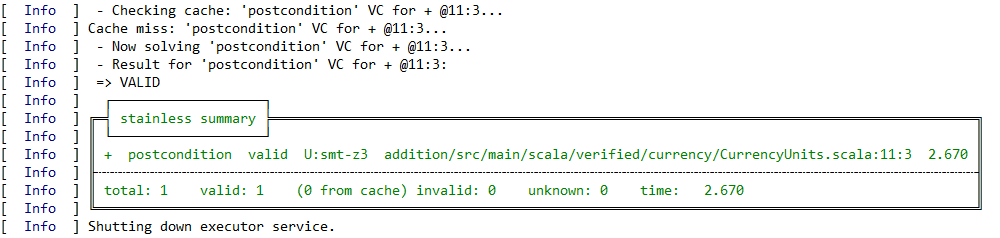
\includegraphics[width=\textwidth]{result_output}
	\caption{Output of Stainless verification for addition with 0 of Bitcoin-S-Cores CurrencyUnit}
\end{figure}









\section{Conclusion}
\label{chap:conclusion}

Because of the limitations of the verication tool, we could only
verify a rewritten version of the original Bitcoin-S code.  So we can
not guarantee the correctness of the addition of Satoshis with zero in
Bitcoin-S.  Not all changes we made were as trivial as the replacement
of objects with case objects.  For these non-trivial changes, as seen
for example the bound check in section \ref{sec:bound_check}, we
cannot say whether they are equivalent to the original implementation
or not.

So code should be written specically with formal verication in mind,
in order to successfully verify it.  Otherwise, it needs a lot of
changes in the software because verification is mathematical and the
current software is written mostly in object-oriented style.  Software
written in the functional paradigm would be much easier to reason
about.

Thus, either Stainless must find ways to translate more of built-in
object-oriented patterns of Scala to their verification tool or
developers must invest more in functional programming.

Also, we found that trying to verify code reveals bugs as shown in
section \ref{sec:bugfix}.  Finally, our work led to some feedback to
the Stainless developers to improve the tool.

\todo{conclusions: what's future work? how to
  change bitcoin-s? how to extend stainless?}

\bibliographystyle{splncs04}
\bibliography{bibliography}


\clearpage
\appendix




% \section{Extracted Code}
% \label{sec:extracted}

% \subsection{NumberType.scala}
% \lstinputlisting[style=scala]{../code/addition/src/main/scala/reduced/number/NumberType.scala}

% \subsection{CurrencyUnits.scala}
% \lstinputlisting[style=scala]{../code/addition/src/main/scala/reduced/currency/CurrencyUnits.scala}


\section{Code Transformations} 
\label{sec:transform}

Here we see in detail how to transform the bitcoin-s code into the
Scala fragment supported by Stainless. All subsections start with the
Stainless error message(s) and finally a description of the changes we
make to the code.

We claim that all transformations are equivalent in the sense that if
the addition-with-zero property holds for the transformed code, then
it also holds for the code before the transformation.


\subsection{Inheriting Objects}


\begin{lstlisting}[style=stainless]
[ Error  ] number/NumberType.scala:65:1: Objects cannot extend classes or implement traits, use a case object instead
          object Int64 extends BaseNumbers[Int64] {
          ^^^^^^^^^^^^^^^^^^^^^^^^^^^^^^^^^^^^^^^^^...
[ Error  ] currency/CurrencyUnits.scala:33:1: Objects cannot extend classes or implement traits, use a case object instead
          object Satoshis extends BaseNumbers[Satoshis] {
          ^^^^^^^^^^^^^^^^^^^^^^^^^^^^^^^^^^^^^^^^^^^^^^^...
\end{lstlisting}

Here, we can just turn the objects into case objects by literally just
changing the word \texttt{object} into \texttt{case object} on lines
65 and 33 in the two respective files.

That transformation is equivalent. Case objects have some additional
properties (in particular, being serializable) and they inherit from
\texttt{Product} instead of \texttt{AnyRef}, but none of our code
depends on any of that.


\subsection{Abstract Type Members}


\begin{lstlisting}[style=stainless]
[ Error  ] currency/CurrencyUnits.scala:6:3: Stainless doesn't support abstract type members
            type A
            ^^^^^^
\end{lstlisting}

Note that we can not simply replace the unsupported abstract type
member by a (supported) type parameter. The problem is that the
CurrencyUnit class uses one of its implementing classes: Satoshis.

Satoshis would have to instantiate a potential type parameter with
type Int64, so it would extend CurrencyUnit[Int64]. But that is too
specific, because the return type of the \texttt{+}-method would then then be
CurrencyUnit[Int64] not CurrencyUnit[A].

Since we only want to verify the addition of satoshis, and the
Satoshis class overrides A with Int64 anyway, we just remove the
abstract type and set it to Int64.

We remove line 6 and line 22 from CurrencyUnits.scala (to maintain
line numbers we actually replace them with empty lines for now) and in
line 18 we replace A by Int64.


\subsection{Non-Literal BigInt Constructor Argument}


\begin{lstlisting}[style=stainless]
[ Error  ] currency/CurrencyUnits.scala:26:33: Only literal arguments are allowed for BigInt.
            def toBigInt: BigInt = BigInt(toLong)
                                          ^^^^^^
\end{lstlisting}

As described before, the types in the Stainless library are more
restricted than their Scala library counterparts. In particular, the
Stainless BigInt constructor is restricted to literal arguments.


Here we can simply use toBigInt on the field \texttt{underlying}
directly.  So, instead of converting the underlying to Long and back
to BigInt we convert underlying directly to BigInt.

We replace line 26 by
\begin{lstlisting}[style=scala]
def toBigInt: BigInt = underlying.toBigint
\end{lstlisting}

This is an equivalent transformation: the only thing that might go
wrong in the detour via \texttt{Long} is that the BigInt underlying
Int64 in turn underlying Satoshis does not fit into a Long. However,
the only constructor of Int64 ensures exactly that.

\subsection{Self-Reference in Type Parameter Bound}

\begin{lstlisting}[style=stainless]
[ Error  ] number/NumberType.scala:8:30: Unknown type parameter type T
          sealed abstract class Number[T <: Number[T]] {
                                        ^^^^^^^^^^^^^^
\end{lstlisting}

Stainless does not currently support a class with a type parameter
with a type boundary that contains the type parameter itself. We opened an
issue \cite{Stainless:issue519} on the Stainless repository and the
Stainless developers have targeted Stainless version 0.4 to support
such self-referential type boundaries.

For now, since our code only uses Number with type parameter T
instantiated to Int64, we just remove the type parameter and replace
it by Int64. We respectively replace lines 8, 44 and 49 by
\begin{lstlisting}[style=scala]
sealed abstract class Number {
\end{lstlisting}

\begin{lstlisting}[style=scala]
sealed abstract class SignedNumber extends Number
\end{lstlisting}

\begin{lstlisting}[style=scala]
sealed abstract class Int64 extends SignedNumber {
\end{lstlisting}

and replace T by Int64 in lines 25-27.


\subsection{Missing Member \texttt{bigInteger} in BigInt}


\begin{lstlisting}[style=stainless]
[ Error  ] number/NumberType.scala:14:22: Unknown call to bigInteger on Number.this.toBigInt (BigInt) with arguments List() of type List()
            def toLong: Long = toBigInt.bigInteger.longValueExact()
                              ^^^^^^^^^^^^^^^^^^^
\end{lstlisting}
\todo{stainless error emssage missing}

The Scala class BigInt is essentially a wrapper around
java.math.BigInteger. BigInt has a member bigInteger which is the
underlying instance of the Java class. The Java class has a method
longValueExact which returns a long only if the BigInteger fits into a
long, otherwise throws exception. Stainless does not support Java
classes and in particular its BigInt has no member bigInteger.

However, our code never calls toLong anymore, so we just remove it. We
replace line 14 in NumberType.scala and line 28 in CurrencyUnits.scala
by an empty line.


\subsection{Type Member}

\begin{lstlisting}[style=stainless]
[Warning ] number/NumberType.scala:9:3: Could not extract tree in class: type A = BigInt (class scala.reflect.internal.Trees$TypeDef)
              type A = BigInt
              ^^^^^^^^^^^^^^^
\end{lstlisting}

Our version of Stainless does not support type members. We just
replace all occurrence of A with BigInt, since A is never overwritten
in an implementing class.

We remove line 9 in NumberType.scala and replace A by BigInt in lines
12, 25, 33 and 50.

In the mean time Stainless has implemented support for type member
\cite{Stainless:pull470}.  Since version 0.2 verification should
succeed without this change.



\subsection{Missing Bitwise-And Method on BigInt}

\begin{lstlisting}[style=stainless]
[ Error  ] number/NumberType.scala:34:14: Unknown call to & on result (BigInt) with arguments List(Number.this.andMask) of type List(BigInt)
              require((result & andMask) == result,
                      ^^^^^^^^^^^^^^^^
\end{lstlisting}

Contrary to Scala BigInt, the Stainless BigInt class does not support
bitwise operations, in particular not the \&-method for bitwise and.

The bitwise and with the andMask on line 34 is a bounds check.  It
checks if the result parameter is in range of the specified type,
which in our case is the hard coded Int64.

So, we replace the \& mask with a check whether the result
is in range of Long.MinValue and Long.MaxValue, because Int64 has the
same 64-bit range as Long.  

We replace lines 34-35 by the following, squeezed into two lines to
preserve line numbers. Note that the BigInt constructor requires a
literal:

\begin{lstlisting}[style=scala]
require(result <= BigInt("9223372036854775807")  
  && result >= BigInt("-9223372036854775808"),
      "Result was out of bounds, got: " + result)
\end{lstlisting}


\todo{kai here we do not know if it changes semantic. ramon: oh, we don't?}



\subsection{Inner Class in Case Object}

\begin{lstlisting}[style=stainless]
[Warning ] number/NumberType.scala:66:3: Could not extract tree in class: case private class Int64Impl extends Int64 with Product with Serializable {
...
[Warning ] } (class scala.reflect.internal.Trees$ClassDef)
              private case class Int64Impl(underlying: BigInt) extends Int64 {
              ^^^^^^^^^^^^^^^^^^^^^^^^^^^^^^^^^^^^^^^^^^^^^^^^^^^^^^^^^^^^^^^^...
...
[Warning ] currency/CurrencyUnits.scala:42:3: Could not extract tree in class: case private class SatoshisImpl extends Satoshis with Product with Serializable {
...
[Warning ] } (class scala.reflect.internal.Trees$ClassDef)
              private case class SatoshisImpl(underlying: Int64) extends Satoshis
              ^^^^^^^^^^^^^^^^^^^^^^^^^^^^^^^^^^^^^^^^^^^^^^^^^^^^^^^^^^^^^^^^^^^
\end{lstlisting}

Stainless does not support inner classes in a case object. Bitcoin-s
uses this a lot to separate the class \todo{ramon: i don't understand} from its implementation.

This is easy to fix. We just move the inner classes out of the case objects. They do
not interfere with any other code.

We remove lines 66-71 in NumberType.scala and insert them at the end of the file.
We remove line 42 in CurrencyUnits.scala and insert it at the end of the file.


\subsection{Message Parameter in Require}

\begin{lstlisting}[style=stainless]
[Warning ] number/NumberType.scala:67:3: Could not extract tree in class: scala.this.Predef.require(Int64Impl.this.underlying.>=(math.this.BigInt.long2bigInt(-9223372036854775808L)), "Number was too small for a int64, got: ".+(Int64Impl.this.underlying)) (class scala.reflect.internal.Trees$Apply)
          require(underlying >= -9223372036854775808L,
          ^^^^^^^^^^^^^^^^^^^^^^^^^^^^^^^^^^^^^^^^^^^^...
[Warning ] number/NumberType.scala:69:3: Could not extract tree in class: scala.this.Predef.require(Int64Impl.this.underlying.<=(math.this.BigInt.long2bigInt(9223372036854775807L)), "Number was too big for a int64, got: ".+(Int64Impl.this.underlying)) (class scala.reflect.internal.Trees$Apply)
          require(underlying <= 9223372036854775807L,
          ^^^^^^^^^^^^^^^^^^^^^^^^^^^^^^^^^^^^^^^^^^^...
[ Error  ] checkResult$0 depends on missing dependencies: require$1.
\end{lstlisting}

Here the require(condition, message) is used as an assertion: if the
condition is false the fail with message.  Stainless does not support
the message parameter of require.  For the verification we can simply
remove that parameter.



\subsection{Missing Implicit Long to BigInt Conversion}

\begin{lstlisting}[style=stainless]
[ Error  ] inv$4 depends on missing dependencies: long2bigInt$0.
\end{lstlisting}

This error message does not specify a line number and it is not clear
what ``inv'' is. However, the Scala BigInt has implict conversions
from Long and they are missing in the Stainless BigInt.



We replace the two require clauses at lines 67 and following in NumberType.scala

\begin{lstlisting}[style=scala]
  require(underlying >= -9223372036854775808L)
  require(underlying <= 9223372036854775807L)
\end{lstlisting}

by:
\begin{lstlisting}[style=scala]
  require(underlying >= BigInt(-9223372036854775808L))
  require(underlying <= BigInt(9223372036854775807L))
\end{lstlisting}

We also replace lines 76 and 77
\begin{lstlisting}[style=scala]
  lazy val min = Int64(-9223372036854775808L)
  lazy val max = Int64(9223372036854775807L)
\end{lstlisting}

by:
\begin{lstlisting}[style=scala]
  lazy val min = Int64(BigInt(-9223372036854775808L))
  lazy val max = Int64(BigInt(9223372036854775807L))
\end{lstlisting}


\subsection{Missing BigInt Constructor with Long Argument}

\begin{lstlisting}[style=stainless]
[ Error  ] apply$14 depends on missing dependencies: BigInt$0, apply$15.
\end{lstlisting}

Here again, the Scala BigInt has a constructor with a Long argument
which is missing in the Stainless BigInt.

We simply replace the Long values in a BigInt constructor call with a string
literal.

The lines from the previous transformation respectively change into
the following:

\begin{lstlisting}[style=scala]
  require(underlying >= BigInt("-9223372036854775808"))
  require(underlying <= BigInt("9223372036854775807"))
\end{lstlisting}

and

\begin{lstlisting}[style=scala]
  lazy val min = Int64(BigInt("-9223372036854775808"))
  lazy val max = Int64(BigInt("9223372036854775807"))
}
\end{lstlisting}


% \section{Verified Code}
% \label{sec:verified}

% \subsection{NumberType.scala}
% \lstinputlisting[style=scala]{../code/addition/src/main/scala/verified/number/NumberType.scala}

% \subsection{CurrencyUnits.scala}
% \lstinputlisting[style=scala]{../code/addition/src/main/scala/verified/currency/CurrencyUnits.scala}





\end{document}
